% Created 2026-08-13 Thu 15:04
% Intended LaTeX compiler: pdflatex
\documentclass[11pt]{article}
\usepackage[utf8]{inputenc}
\usepackage[T1]{fontenc}
\usepackage{graphicx}
\usepackage{longtable}
\usepackage{wrapfig}
\usepackage{rotating}
\usepackage[normalem]{ulem}
\usepackage{amsmath}
\usepackage{amssymb}
\usepackage{capt-of}
\usepackage{hyperref}
\author{fcalado}
\date{\today}
\title{}
\hypersetup{
 pdfauthor={fcalado},
 pdftitle={},
 pdfkeywords={},
 pdfsubject={},
 pdfcreator={Emacs 29.3 (Org mode 9.6.15)}, 
 pdflang={English}}
\begin{document}

\tableofcontents

\section{CHAPTER TWO "Text Analysis"}
\label{sec:orgf39a35e}

\subsection{Doubt}
\label{sec:orga5d6e95}
1

The novel \emph{Orlando: A Biography} (1928), by Virginia Woolf, famously
opens with an assertive gender designation followed by an immediate
qualification:

\begin{quote}
He---\emph{for there could be no doubt of his sex}, though the fashion of
the time did something to disguise it---. (italics mine, 11)
\end{quote}

2

In order to perform quantitative text analysis on this text, the
standard tasks of "pre-processing" or "cleaning" would evacuate this
sentence of its gender qualification. Cleaning the first sentence not
only would strip it of its pronouns, including the gender assertion in
the first word, "He," it would also cut the em dash immediately
following "He," signaling the entrance of the narrator and his
conspicuous certitude, "---for there could be no doubt of his sex."
Only the following list of words would remain:

3

\begin{quote}
‘could’, ‘doubt’, ‘sex’, ‘though’, ‘fashion’, ‘time’, ‘something’,
‘disguise’
\end{quote}

Text analysis, a process which involves calculating and visualizing
textual patterns, requires transforming the source text into a
computable format. Cleaning the text strips capitalized words,
punctuation, “stop words” (such as articles and prepositions), and
inflections in word endings, all of which are deemed to be
semantically minor, so that they don't affect the analysis of more
substantial features like nouns, verbs, adverbs, and adjectives. Text
analysis requires removing such "minor" elements of language in order
to find connections among more apprently substantial terms.

4

However, the word "He," and the em dash following and accentuating
that "He," is hardly minor in a text that famously interrogates gender
differences and shifts in gender. \emph{Orlando: A Biography}, is a
fantastical novel whose eponymous main character lives 300 years and
inexplicably changes his gender from male to female. Indeed, as Pamela
Caughie puts it, the pronoun and punctuation in the first sentence
effectively announces the book's investment in gender subversion:
"immediately our doubt is aroused\ldots{} The emphasis on an innocent
pronoun makes it suspect" ("Double Discourse" 42).

5

This chapter examines how quantitative text analysis works to analyze
the gender binary by using Woolf’s \emph{Orlando} as a test case. It
explores an experimental approach to text analysis that deconstructs
the gender binary by drawing connections between computer programming
and gender theory. This analysis surfaces a mechanism, specifically a
technical constraint, common to both text analysis and gender
performativity, which is \emph{iteration}. This constraint powers both text
analysis and in gender theory in a logic of repetition which, I argue,
can be harnessed to re-work text analysis procedures in ways that
bring previously suppressed details of language to the surface. The
final section of the chapter thus proposes a text analysis method that
re-signifies the meaning of binary gender terms, of "man" and "woman."
It works within the constrictive structure of iteration, of text
analysis procedures, in order to unmake them from the inside.

\subsection{Falsifiable}
\label{sec:orgd807af1}
1

The history of text analysis as a practice has been traced to many
origins.\footnote{One rendition traces this lineage to Roberto Busa, an Italian
Jesuit priest who authored the first digital condordance, the \emph{Index
Thomisticus} (See Ramsay, Stephen, \emph{Writing Machines}. 2011). Another
prominent scholar, Ted Underwood, traces this practice to Literary
Studies scholars at the intersection of literary studies and social
science, centering the work of marxist scholar Raymond Williams and
feminist scholar Janice Radway (See Ted Underwood, "A Genaeology of
Distant Reading").} My particular version begins with Franco Moretti, whose
seminal book on "distant reading," published as a series of polemical
essays in a collection of the same name in 2008, dominated discussions
of digital humanities and literary studies I was a graduate student.
Distant reading, by Moretti's account, involves counting up textual
features to derive textual patterns and make inferences. It is an
analytical perspective where "distance," he explains, "is a condition
of knowledge" (\emph{Distant Reading} 48).

2

Shortly after the publication of a \emph{New York Times} profile of the
scholar, three of his former students came forward to accuse him of
sexual crimes. The accusations ranged from unsolicited touching to
rape. At the time of the alleged incident, one of his accusers,
Kimberly Latta, was a first-year graduate student.
\begin{quote}
When I was a graduate student at UC Berkeley in 1984-85, my
then-professor Franco Moretti sexually stalked, pressured, and raped
me. He specifically said to me, 'You American girls say no when you
mean yes.'[\ldots{}] I reported him to the Title IX officer [\ldots{}] and he
threatened to ruin my career if I pressed charges against him. He said
he had powerful friends who were attorneys who would ruin my name. I
remained silent for all these years because I was in academia"
(Kimberly Latta "Op-Ed: What Happened?" 2017).
\end{quote}
When the women came forward, Stanford went no further than claiming
they would review the cases. There has been no record of an inquiry,
investigation, or any repercussions for Moretti (Liu, Knowles,
"Harassment, assault allegations against Moretti span three
campuses"). He remains an Emeritus Professor at Stanford.

3

At the time of the alleged assault, Moretti was riding his first wave
of academic celebrity. Invited to teach at Berkeley, he had just
published a collection of essays, \emph{Signs Taken For Wonders: On the
Sociology of Literary Forms} (1983), a book which already expressed
his polemical style and sowed the roots of his quantitative approach
to studying literature. The first essay, "The Soul and the Harpy,"
takes traditional literary criticism as its target, critiquing the
methodology of close reading. According to Moretti, close reading is
overly subjective, turning the critic to a kind of "Narcissus", "whose
only pleasure lay in contemplating his own reflection (“Soul” 14). He
proposes an alternative, "falsifiable criticism," a methodology that
pursues answers which are irrefuatable. He asserts that,

\begin{quote}
"The day criticism gives up the battle cry ‘it is possible to
interpret this element in the following way,’ to replace it with the
much more prosaic ‘the following interpretation is impossible for such
and such a reason,’ it will have taken a huge step forward on the road
of methodological solidity." (“Soul” 22)
\end{quote}
Moretti implicitly aligns literary criticism with methodologies from
the social sciences, methods which are traditionally described as
"reproducible."\footnote{Sarah Cohen-Boulakia, Khalid Belhajjame, Olivier Collin, Jérôme
Chopard, Christine Froidevaux, Alban Gaignard, Konrad Hinsen, Pierre
Larmande, Yvan Le Bras, Frédéric Lemoine, Fabien Mareuil, Hervé
Ménager, Christophe Pradal, Christophe Blanchet, Scientific workflows
for computational reproducibility in the life sciences: Status,
challenges and opportunities, Future Generation Computer Systems,
Volume 75, 2017, Pages 284-298, ISSN 0167-739X
\url{https://doi.org/10.1016/j.future.2017.01.012}.} Reproducible methodologies obviate the risk of
alternative interpretations by supplying conclusions that are, in
Moretti's words, “coherent, univocal, and complete” (“Soul” 21).

4

Twenty years later, falsifiable criticism finds an ideal toolset in
quantitative practices. Rather close attention to individual samples,
quantification counts patterns of specific features across wide swaths
of text. As we will see below, it simplifies text into workable units,
which is the basis for higher levels of computation. These simple and
workable units, at large scales, enable ambitious interpreptations. As
Moretti explains, "If we want to understand the system in its
entirety, we must accept losing something. We always pay a price for
theoretical knowledge" (\emph{Distant Reading} 49).

5

As a young graduate student, I found Moretti's writing both striking
and alluring. He is an assertive writer, using mostly short sentences
that give his prose a plucky rhythm. Moreover, despite drawing from
disparate fields of knowledge, such as evolutionary theory, systems
theory, and Marxism, his arguments seem to circle methodically around
a drain so that, as long as you're following him, there appears to be
no alternative. Paragraphs begin with sentences like,

\begin{quote}
So, the market selects the canon. (69)

So. As novelistic forms travel through the literary system, their
plots are (largely) preserved, while their styles are (partly)
lost---and replaced by 'local' ones. (134)

What did the birth of a consumer society mean for the European novel?
More novels, less attention. (175)

The major metamorphosis of eighteenth-century titles is simple: in the
space of two generations, they become much, much shorter. (182)

As the market expands, titles contract; as they do that, they learn to
compress meaning; and as they do \emph{that}, they develop special
'signals' to place books in the right market niche. (204)
\end{quote}

These sentences, taken from mostly different essays in \emph{Distant
Reading}, synthesize arguments and evidence from previous paragraphs.
They are more summary of previous points than new argumentation. Yet,
their apparent solidity, the lack of a subjective "I" to ground them,
strikes me as suspect. It showcases Moretti's characteristic way of
transforming inferences, premises, and hypotheses into declarative
statements, stating a claim or hypothesis as an objective or
self-evident fact. And moreover, they suppress the possibility of
alternative views---falsifying them before they even have the space to
speak.\footnote{The faith in the falsifiable, in the power of supposedly
objective processes of quantitative computation, is powerful and
contagious. It spreads even to those who believe that it has no place
in Literary Studies. A controversial detraction by Nan Z. Da claims
there is a "fundamental mismatch between the statistical tools that
are used and the objects to which they are applied"--that is, to
literary objects (620, 601). Yet, despite her oppositional stance
toward quantitative tools, Da has something in common with those who
champion them: she \emph{agrees} about the objectivity of their procedures.
As Ben Schmidt points out, “Far more than anyone I’ve seen in any
humanities article, she asserts that scientists do something arcane,
powerful, and true" (Schmidt, "A computational critique of a
computational critique of computational critique."). Despite their
vastly different views on the role of quantitative methods for
studying literature, Da and Moretti appear to agree that these methods
ought to provide results that are, at the very least, reproducible.}

6

In one of the more famous essays from \emph{Distant Reading}, "Style, Inc.:
Reflections on 7000 Titles (British Novels, 1740-1850)" Moretti uses
text analysis to study the market for British novels from 1740 - 1850.
Here, he explores what titles, which shorten in length over the
decades, reveal about the rise and fall of certain genres in the
market. He outlines his analytical process:
\begin{quote}
[F]irst, I describe a major metamorphosis of eighteenth-century
titles, and try to explain its causes; next, I suggest how a new type
of title that emerged around 1800 may have changed what readers
expected of novels; and finally, I make a little attempt at
quantitative stylistics, examining some strategies by which titles
point to specific genres. Three sections, three pieces in the large
puzzle of the literary field. (\emph{Distant Reading} 181-2; emphasis mine)
\end{quote}
Moretti's critical method involves posing hypotheses, assembling and
analyzing data, making inferences, and occasionally, reframing the
original hypotheses. Yet, he repeatedly understates his interpretive
moves at each stage of his analysis: “try to explain,” “suggest,”
"make a little attempt." As Stephen Ramsay points out, Moretti
presents his own insights as a description of reality, as if "data is
presented to us\ldots{} not as something that is also in need of
interpretation" (Ramsay, \emph{Reading Machines} 5). Moretti misrepresents
the role that inferential thinking plays in some truly fascinating
insights, for example, that titles function as a proxy for market
forces, as "a code, in the market\ldots{} where the novel as language meets
the novel as commodity" (\emph{Distant Reading} 181).

8

Particularly, as Lauren Klein points out, distant reading can
overlook details which are necessary to cultural critique. In a talk
titled "Distant Reading After Moretti," Klein explains,
\begin{quote}
[I]t’s not a coincidence that distant reading does not deal well with
gender, or with sexuality, or with race. Gender and sexuality and race
are precisely the sorts of concepts that have been exposed and
interrogated by attending to non-dominant subject positions. And like
literary world systems, or "the great unread," the problems associated
with these concepts, like sexism or racism, are also problems of
scale, but they require an increased attention to, rather than a
passing over, of the subject positions that are too easily (if at
times unwittingly) occluded when taking a distant view.
\end{quote}

Klein's own work tracing these elements proves how careful attention
to what is minor or oblique can surface previously suppressed stories.
In one project, Klein uses network analysis methods to bring forth the
"ghost" of a previously obscured subject, James Hemmings. Hemmings, a
slave who worked for Thomas Jefferson until he could negotiate his
freedom, appears in brief references in Jefferson's correspondence. By
marking up and visualizing these oblique references, Klein "render[s]
visible the archival silences implicit in our understanding of chattel
slavery today" (665). Her work demonstrates that the details of
Hemmings's life, which are deeply distributed in the correspondence
data, requires a kind of reading that is close and careful.

10

The ambition to grasp large swaths of literary history\footnote{Distant reading is permeated by great ambition. In
\emph{Macroanalysis: Digital Methods and Literary History} (2013), Matthew
Jockers "ask[s] very big questions\ldots{} regarding how literary trends
are employed over time, across periods, within regions"; In \emph{Distant
Horizons: Digital Evidence and Literary Change} (2020) Ted Underwood
traces the "larger arcs of literary change that have remained hidden
from us by their sheer scale." Most recently, [ADD RECENT EXAMPLES,
PREFERABLY MONOGRAPHS?].} may be a
proxy for avoiding certain kinds of cultural critique. The proxy
functions through an amplification and valorization of what is
seemingly objective--for example, the counting of words. With word
counts and their resulting graphs and charts doing the work of
analysis, one finally closes down the pesky, subjective
interpretations asssociated with close reading. As Moretti says, "we
know how to read texts, now let's learn how \emph{not} to read them"
(\emph{Distant Reading} 48).

More than avoidant, I want to argue, this faith in the falsifiable is
intellectually coercive. It can be a way of silencing less prominent
or otherwise inconvenient views. It marshalls seemingly irrefutable
evidence, word counts, for example, and places them in support of a
supposedly "objective" interpretation. It is an imposition of a view
from the top. And coming from the top, it functions like other
hierarchies of power, like academic prestige. Like when an older,
accomplished male professor gets away with telling a young, female
graduate student that "You American girls say No when you mean Yes".

11

Since Moretti, however, there have been many liteary scholars that
push back against the apparent objectivity of reproducible methods.
Ted Underwood, for example, explains that "algorithms are actually bad
at being objective and rather good at absorbing human perspectives
implicit in the evidence used to train them" (“Machine Learning and
Human Perspective” 92). Underwood creates what he calls "perspectival
models" of literary data, where models represent different databases
associated with different "perspectives." In one project, on studying
gender in novels, Underwood uses a binary classification algorithm to
cluster terms that male and female writers, two "perspectives," tend
to associate with either gender. From the results, he creates a chart
which visualizes the differences between male and female writers and
their treatment of gender.

\begin{center}
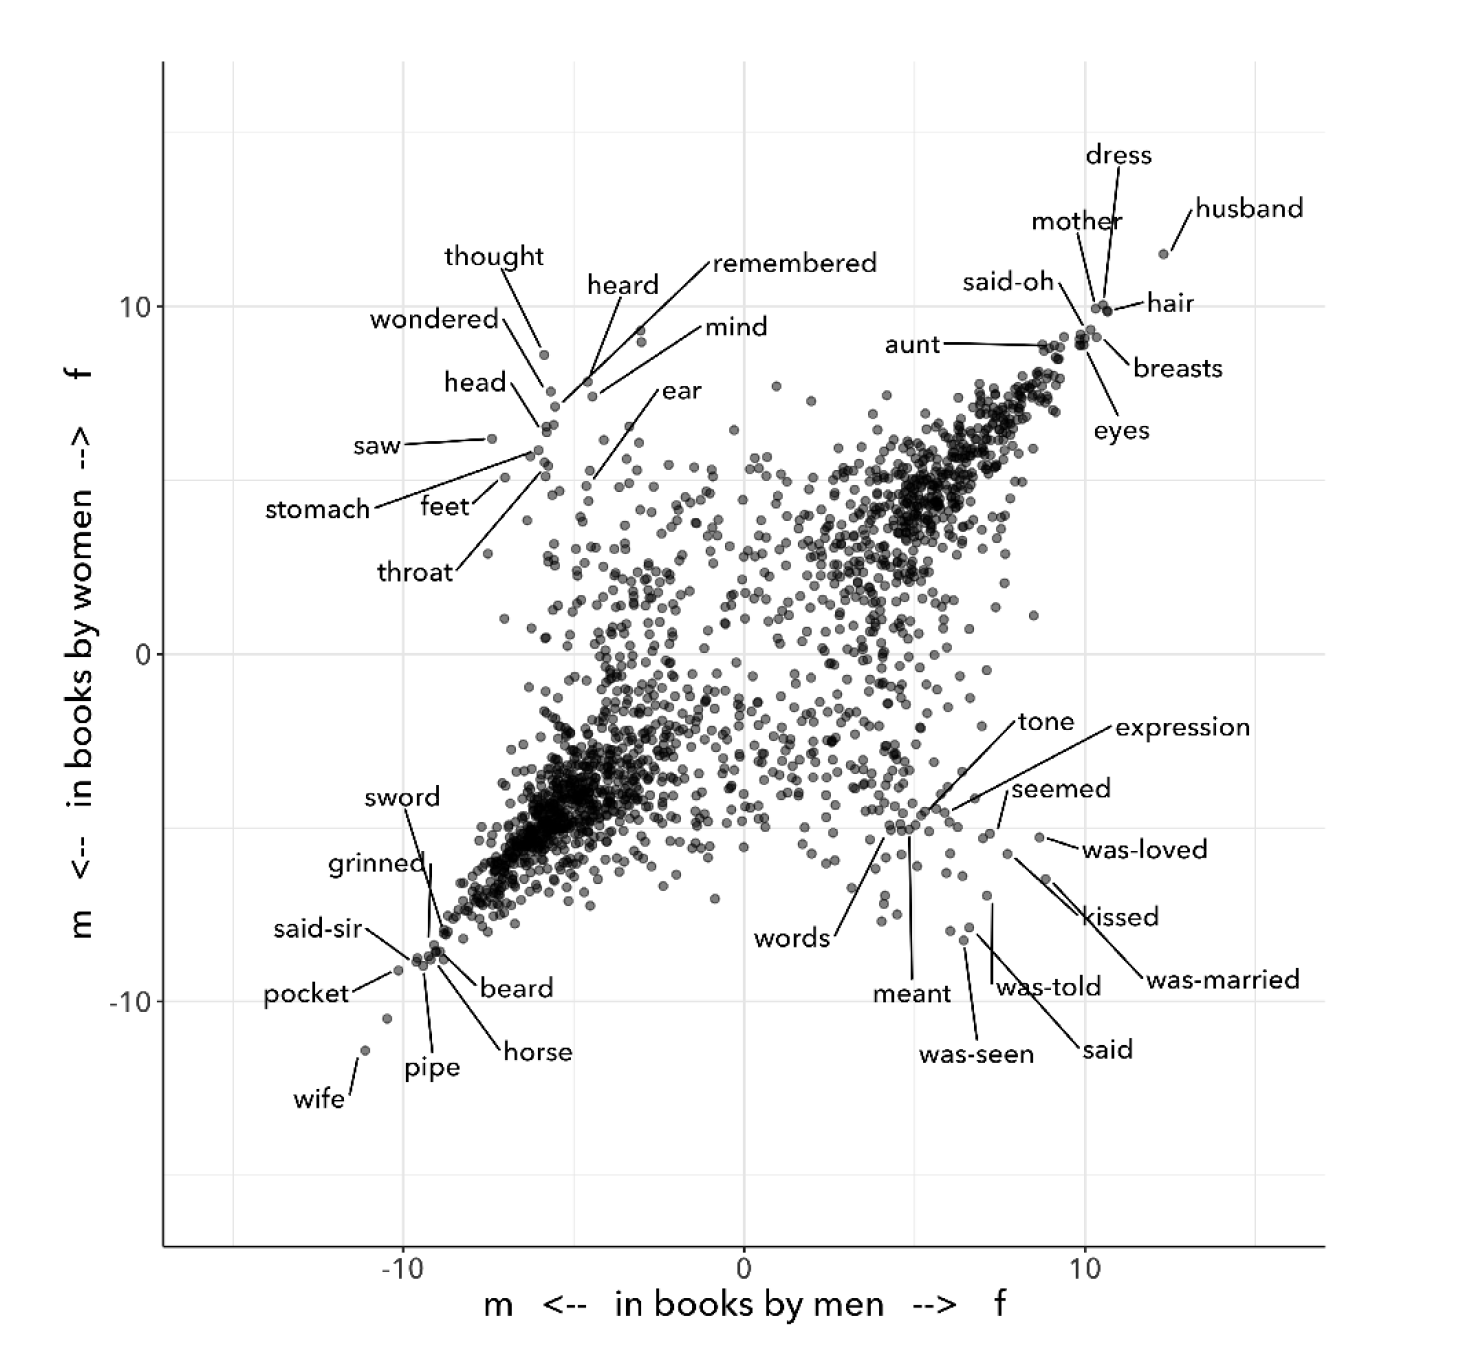
\includegraphics[width=.9\linewidth]{./images/underwood.png}
\end{center}

In this chart (see Fig. 1), there are two diagonals. The diagonal
moving from the bottom-left to top-right corner represents where the
genders agree on gendered terms. The bottom-left shows agreement on
terms used to describe the male gender ("pocket", "grinned"), and the
top-right shows agreement on the female gender ("eyes," "mother"). The
opposite diagonal, running from the top-left to bottom-right corners,
shows disagreement. The top-left shows terms that each gender tends to
use to describe their own gender ("wondered", "mind") and the
bottom-right shows terms that each gender uses to describe the
opposite gender ("meant", "kissed"). The chart, according to
Underwood, shows two \emph{perspectives} on gender--the male and the
female. Rather than making claims to gender in an objective sense, it
dramatizes a perspectival shift between the two genders.

12

Underwood's methodology, as he himself admits, reinscribes the gender
binary. When explaining the diagram, he predicts that "gender
theorists will be frustrated by the binary structure of the diagram\ldots{}
I needed a simple picture, frankly, in order to explain how a
quantitative model can be said to represent a perspective" (“Machine
Learning and Human Perspective” 98). This reinscription of the "binary
structure" happens not only in the choice of model, a classification
(i.e. binary) model which makes predictions on a yes/no or, in this
case, a male/femal scale. It also happens with the choice in
visualizing the results in a way that places male and female genders
in opposition. The diagonal going from the bottom-left to the
top-right, which finds similarity between the genders, reinforces a
stereotypical active/passive binary (among other binaries) between men
and women. Similarly, the diagonal going from the top-left to the
bottom-right, although based on agreement between the genders and
their relationships to themselves, nonetheless imposes an \emph{opposition}
between how male and female authors describe each other. The graph
effectively instantiates its implicit assumption that male and female
writers will oppose the other by visualizing this as a feature.

Beyond this reification of the gender binary, however, Underwood's
visualization effectively deploys the gender binary \emph{as a model} for
proving the value of quantitative methods. In order for his experiment
to take place, the gender binary is a necessary presumption, a "ground
truth," that makes the choice of a classification model appear
appropriate. In other words, before he even constructs the diagram,
gender roles have been already manufactured into opposition.

14

There certainly are provocative reasons to study gender as a binary
system. But when driven by the interest of posing one gender \emph{against}
another, ("how to distinguish between male and female writers?") such
experiments effectively \emph{reify} the binary.

Which is not, I believe, as interesting as work that explicitly
deconstruct these categories (and categorization) in the first place.
For example, Laura Mandell studies gender through genre. Mandell
deploys the popular stylometry measurement, “Burrow’s Delta,” which
visualizes the “distance” between writing styles by creating branches
("deltas") between different texts. She finds that Mary
Wollstonecraft's style is shared across comparable male writers like
William Godwin and Samuel Johnson: “Wollstonecraft’s sentimental
anti-Jacobin novels most resemble Godwin’s sentimental anti-Jacobin
novels… whereas her essays most resemble Johnson’s writings” ("Gender
and Cultural Analytics:: Finding or Making Stereotypes?" par. 29). Her
analysis creates new categories that draw gender into genre--squaring
the gender binary. She creates doubly refracted categories like, "men
writing as men," "women writing as women," "women writing as men,"
"men writing as women" (par. 35).

15

Applying text analysis to racial categories, Edwin Roland and Richard
Jean So explore whether a machine can correctly identify the race of a
novel's author. The point, they are careful to say, is not to test
whether the machine is correct, but to examine how the categories
themselves are constructed. As they explain, "the machine simply
measures the robustness of the social constructedness of these given
categories and points out what gives them such vigor" ("Race and
Distant Reading" 69). Analyzing a large corpus of novels by white and
black authors, So and Roland find that black authors generally display
more varied vocabulary than white authors. From this result, they
infer that White authorship only coheres \emph{as a category} against the
variance of Black authorship. In other words, White authorship is only
visible as a category when it is compared to Black authorship, which
displays overall more varied uses of language forms.

Interestingly, this quantitative exercise points Roland and So toward
a peculiarity in the results: that the algorithm wrongly categorizes
Black-authored novel, James Baldwin's \emph{Giovanni’s Room} (1956), as
being written by a White author. This misclassification is due to a
single word--"appalled"--whose usage, according to the model, has
generally been a signal of White authorship. The term only occurs once
in the text, in an early scene where the narrator David describes his
strained relationship to his father: “I did not want to be his buddy.
I wanted to be his son. What passed between us as masculine candor
exhausted and appalled me” (Rpt. in Roland, So 71; emphasis mine).
Given the connotation of whiteness in "appalled" and its middle French
root, “apalir” (to grow pale), Roland and So explain that this
term--which emerged as a result of the computer's mistake--enables
their analysis to coordinate gender to race: “the moment David
develops a troubled relationship to normative masculinity [as] also
the moment he becomes ‘White’” (71). Rather than reify racial
categories, this computational experiment points out that they are
constructed on certain assumptions.

16

So and Roland began with the binary form, the binary categories of
Black/White, but they ended with its fracturing. This fracturing,
evident in the computer's misclassification of authorship in
\emph{Giovanni's Room}, leads to a reading which coordinates race with
gender and sexuality. This "queering the machine’s color line," the
authors explain, opens up new readings of intersectionality in the
novel which "in their current form, our data and model are not robust
enough to handle" (72). Rather than reproducible, this method is
fracturing and refractive, both reflecting and corrupting the
constructed nature of binary structures back at the critic. It brings
us closer to the methodology that I outline in the next section,
\emph{iteration}.

\subsection{Iteration in gender}
\label{sec:orgad602d7}
1

Some text analysis projects take the language of performance and
qualities of the performative to describe and conceptualize their
methodologies. For example, Mandell's project takes the behavioral
quality of gender performativity and applies it to genre, asserting
that both gender and genre "are\ldots{} highly imitatable," so that "anyone
can adopt gendered modes of behavior, just as anyone can write in
genres stereotypically labeled M/F" (par. 30). In Computational
Literary Studies (CLS), Bode operationalizes the "performative" to
describe the analytical act itself, which intervenes and becomes
inseparable from the object of analysis. "Peformativity," they argue,
is "attuned to the coconstitution of computational methods and
objects" ("What's the Matter with Computational Literary Studies").
Their research explores how "meaning is not carried by texts but
produced in situated interactions between readers, texts and
contexts," including computational tools.\footnote{Bode, Katherine. “Data beyond representation: From computational
modelling to performative materiality.” MLA Convention, Seattle, 10
January 2020.
\url{https://katherinebode.wordpress.com/home/mla-convention-2020/}} From the field of
Computational Humanities, Kent K. Chang, Anna Ho and David Bamman cite
performativity as motivation to computationally "measure subversion"
in TV show dialogue, to predict whether samples of a TV show, \emph{The Big
Bang Theory}, are queer-coded.

2

My examination surfaces a particular mechanism that drives
performativity---which is the mechanism of iteration, a process of
repetition by which gender performativity both operates, and by which
it can also be exploited. This focus on iteration addresses a common
misreading of performativity, that it denotes a series of acts that
can be imitated at will. Indeed, Butler's follow up to \emph{Gender
Trouble: Feminism and the Subversion of Identity} (1990), which is
\emph{Bodies that Matter: on the Discursive Limits of Sex} (1996), aimed to
clarify how performativity is compulsory, bounded on all sides by
social norms in ways that delimit a subject's agency. In \emph{Bodies that
Matter}, Butler explains that gender performativity is a
pre-determined procedure that \emph{constitutes} subjectivity: "there is no
subject who decides on its gender\ldots{}. on the contrary, gender is part
of what decides the subject" (ix).

That being said, performativity can be subverted, according to Butler.
Rather than through individual will, however, subversion comes from
manipulating this iterative process. This manipulation brings
something something unexpected and extraneous into the performance,
while staying within the very terms of that performance, as I explain
below.

3

To understand how this possibility for subversion works, one must
first understand how the performative is constituted, according to
Butler. Essential to Butler's thinking is the poststructuralist
feminist theorist, Luce Irigaray and her methodology for critiquing
masculine language in her book, \emph{The Sex Which Is Not One} (Irigaray
23). Irigaray argues that philosophers like Plato, Aristotle,
Descartes, and others, represent the feminine through masculine terms,
"on the basis of masculine parameters," which is through the binary
form (18). Irigaray argues that the Male/Female binary (among other
binaries) effectively \emph{precludes} the representation of the other
term, the feminine. Moreover, this exclusion of the feminine, as it
happens, effectively \emph{produces} another feminine within the terms of
the masculinist system. In other words, the feminine which has been
excluded from the system, which must be excluded in order for that
system to work, into what Butler calls the "constitutive outside,"
makes possible the creation of the inner, "domesticated" feminine.
This feminine, which is "unspeakable" and unrepresentable, is the
\emph{matter} from which the Male/Female binary comes into intelligibility.

4

The excluded feminine is, Butler explains, a matrix. In Butler's
words,

\begin{quote}
every explicit distinction takes place in an inscriptional space that
the distinction itself cannot accomodate. Matter as a \emph{site} of
inscription cannot be explicitly thematized\ldots{} [this] inarticulate
"matter" designates the constitutive outside of the Platonic economy;
it is what must be excluded for that economy to posture as internally
coherent (emphasis original, 12-13).
\end{quote}

This \emph{matrix}, this "inscriptional space", which cannot be
articulated, draws simultaneously from a classical analogy between the
form/matter and masculine/feminine, in the Aristotelian tradition, and
from the etymological association between the feminine as \emph{mater}
(mother). It is the generative material for all life, from which all
distinctions of male/female can emerge.

5

But where is this excluded feminine? If it indeed "cannot be
thematized," could it possibly be invoked, without subscribing itself
to the ruling, masculine structure? 

6

The answer invovles breaking open performativity's process of
repetition. Performativity relies on repetition, a perpetual
re-creation of the norm, which effectively produces and re-produces
power structures. As Butler explains, "performativity must be
understood not as a singular or deliberate 'act,' but, rather, as the
\emph{reiterative} and citational practice by which discourse produces the
effects that it names" (xii). According to Butler, it is through
performativity that "sexed" bodies emerge: "'Sex' is not a simple fact
or static condition of a body, but a process whereby regulatory norms
materialize 'sex' and achieve this materialization through a forcible
reiteration of those norms" (xii). What appears as physical or
biological category is actually a "sedimentation" formed through
repetition.

7

This sedimentation, whereby meaning is signified and re-signified
endlessly, is never complete. Categories like sex, as Butler explains,
require constant repetition:

\begin{quote}
This "being a man" and this "being a woman" are internally unstable
affairs. They are always beset by ambivalence precisely because there
is a cost in every identification, the loss of some other set of
identifications, the forcible approximation of a norm one never
chooses, a norm that chooses us. (86)
\end{quote}

By this "cost in every identification," Butler means all of the
identifications which are effectively rejected when one makes a claim
to identity. Repetition stabilizes gender identity against a field of
potential exclusions. And it is these exlusions which will come back
to haunt the coherence of the identity. 

8

This mechanism of repetition, which Butler calls "iteration," creates
an excluded field of possible identities. As Butler explains, every
"identification takes place through a repudiation which produces a
domain of abjection" (xiii). However, these repudiated, disavowed
identities offer "a field of disruptive possibillities," where terms
may draw from rejected meanings to be resignified. Such
resignfications destabilize the stability of the claimed identity,
"threaten[ing] to expose the self-grounding presumptions of the sexed
subject" (xiii).

9

Butler offers an example with the term "queer," which is a term that
harnesses its own history of repudiation for political purposes. The
adoption of this term by Gay and Lesbian activism in the 80s and 90s
"resignif[ies] the abjection of homosexuality into defiance and
legitimacy" (Butler xxviii). This turning of abjection into legitimacy
shows how one attains some kind of agency even within the terms of
subjection.

\begin{quote}
The compulsion to repeat an injury is not necessarily the compulsion
to repeat the injury in the same way or to stay fully within the
traumatic orbit of that injury. The force of repetition in language
may be the paradoxical condition by which a certain agency---not
linked to a fiction of the ego as master of circumstance---is derived
from the impossibility of choice. (183)
\end{quote}

It is through the repetition of repudiated meanings, which necessarily
draw from insulting and/or painful pasts, come to alchemize new
significations. If a repudiated meaning, a "troubling return," is
repeated enough times, Butler argues, the stability of the original
identity will be brought into question. The paradox is that what
appears to be a cyclical or even robotic behavior takes on an agentic
capacity.

10

Returning to Irigaray, Butler explains that Irigaray achieves a kind
of subversion of the masculinist system of representation by "mim[ing]
philosophy\ldots{} and, in the mime, tak[ing] on a language that
effectively cannot belong to her" (12). Butler cites a passage where
Irigaray "mimes" the style of Plato. By taking on Plato's language,
Irigaray "performs a repetition and displacement of the phallic
economy" (Butler 18). In an interesting double mimicry, with Butler
mimicking Irigaray mimicking Plato, Butler writes,

\begin{quote}
I will not be a poor copy in your system, but I will resemble you
nevertheless by miming the textual passages through which you
construct your system and showing that what cannot enter it is already
inside it (as its necessary outside), and I will mime and repeat the
gestures of your operation until this emergence of the outside within
the system calls into question its systematic closure and its
pretension to be self-grounding. (18)
\end{quote}

Irigaray undermines the authority of the masculine through repetition,
"cit[ing] Plato again and again," in a re-iterative practice (18).
This practice has a cumulative effect, which is to "expose precisely
what is excluded" from the system, and "to reintroduce the excluded
into the system itself" (Butler 18). Through iteration, one displaces
the expectation, the norm, to suggest something else. This something
else, however, is not meant to replace the norm, but to undermine its
pretensions. Butler explains that "This is a taking of his [Plato's]
place, not to assume it, but to show that it is \emph{occupiable}\ldots{} a kind
of overreading which mimes and exposes the speculative excesses in
Plato (emphasis original, 11).

11

The mechanism of iteration aims to destabilize the ruling system from
within. And this is where Butler's theory is often misunderstood. For
example, Chang et. al's text analysis project, cited above, argues
that "subversion" occurs through two straight characters whose
dialogue expresses homosexual innuendo in a popular TV show, \emph{The Big
Bang Theory}. The authors claim that "an undercurrent of emotional
intimacy and dependency\ldots{} challenges the rigid boundaries of what is
considered acceptable" on the show (Chang et al., 10). However,
according to Butler, subversion requires a destabilization from the
inside in a way that occupies and displaces the expected norm. These
characters, however much they are queer-coded, ultimately remain
within hetersexual relationships. The show thus reproduces what Butler
describes as "drag as high het entertainment":

\begin{quote}
[T]hink of Julie Andrews in \emph{Victor, Victoria} or Dustin Hoffmann in
\emph{Tootsie} or Jack Lemmon in \emph{Some Like It Hot} where the anxiety over
a possible homosexual consequence is both produced and deflected
within the narrative trajectory of the films. These are films which
produce and contain the homosexual excess of any given drag
performance, the fear that an apparently heterosexual contact might be
made before the discovery of a nonapparent homosexuality. (85)
\end{quote}

Butler explicitly stipulates against "forms of drag that heterosexual
culture produces for itself," which effectively prop up heterosexual
regimes. Rather than queerness as subversion, this is closer to what
Irigaray describes as the "domesticated" element. In this case,
potential subversion is domesticated by humor, which "produce[s] and
contain[s] the homosexual excess" of the show.

12

Subversion then, is a kind of \emph{occupation} of meaning that works
toward displacement through resemblance. It occurs by way of
overreading, as Irigaray does with her mimicry of Plato's style. The
key is repetition, or more precisely, \emph{iteration}, a continual miming
of the authorizing norm. Through the iterative process, one brings
back again and again the repudiated meaning: through subservience,
insubordination.

\subsection{Iteration in python}
\label{sec:orgfdcd911}

1

As with gender theory, iteration is a core concept in programming.
Iteration means repeating the same action to each bit of data in a
collection of data. For text analysis in particular, it is immensely
useful. 

2

For example, the looping mechanism effectively "cleans" a text one
word at at time. Cleaning typically involves removing elements like
articles and prepositions whose high frequencies would obstruct
quantitative analysis.\footnote{Elements that are highly frequent, like articles,
prepositions, and even pronouns, can drown out other terms which are
considered more substantial, like nouns and verbs. Additionally,
irregular cases also need to be standardized, because capital letters
would count toward different words (for example, "talk" and "Talk"
would be considered two different words). For similar reasons, word
endings and inflections like plural forms (endings in "s") and tenses
('walked', 'walks' or 'walking') are converted into a root form.} Using a loop, a person may \emph{iterate}
through each word in a text, check whether it needs to be "cleaned,"
and then perform a set of cleaning actions.

\begin{verbatim}
clean = [] 
for word in text:
    if word.isalpha():
        clean.append(word.lower())
\end{verbatim}

The first line of code here creates an empty placeholder, \texttt{clean},
where words will be saved in their clean form. Then, the next line
begins the \texttt{for loop}, which specifies a series of actions to execute
on each word in the text, in this case, in Woolf's novel, \emph{Orlando}.
The loop will first take the first word, "He," and then the second
word, which is in this case a punctuation, an em dash, "---," and
next, the preposition "for," and so on. The third line contains a
filter, \texttt{isalpha()}, which checks if the word is comprised of only
alphabetic characters (i.e. it is not a number or punctuation). If the
word is alphabetic, it passes the filter (at this point, the em dash
would fail this requirement, and wouldn't pass to the next line). At
the next line, the word is lowercased, \texttt{lower()} and finally added to
the empty list, \texttt{clean}.

The loop runs over each word in \emph{Orlando}, one by one. When the loop
is done running, the final list of words in \texttt{clean} will contain
alphabetic and lowercased letters. For example, here is what remains
of the first sentence of the novel, with all words in are lowercase,
and no punctuation.


\begin{verbatim}
['he', 'for', 'there', 'could', 'be', 'no' 'doubt', 'of', 'his' 'sex',
 'though', 'the' 'fashion', 'of', 'the' 'time', 'did', 'something',
 'to', 'disguise', 'it']
\end{verbatim}



3

The next step in cleaning is to remove overly frequent words called
"stop words." These words consist of prepositions, articles, pronouns,
and auxiliary verbs---all of which are deemed to be semantically
insubstantial relative to their frequency.

\begin{verbatim}
stop-words = ["i", "me", "my", "myself", "we", "our", "ours",
              "ourselves", "you", "your", "yours", "yourself",
              "yourselves", "he", "him", "his", "himself", "she", "her",
              "hers", "herself", "it", "its", "itself", "they", "them",
              "their", "theirs", "themselves", "what", "which", "who",
              "whom", "this", "that", "these", "those", "am", "is", "are",
              "was", "were", "be", "been", "being", "have", "has", "had",
              "having", "do", "does", "did", "doing", "a", "an", "the",
              "and", "but", "if", "or", "because", "as", "until", "while",
              "of", "at", "by", "for", "with", "about", "against",
              "between", "into", "through", "during", "before", "after",
              "above", "below", "to", "from", "up", "down", "in", "out",
              "on", "off", "over", "under", "again", "further", "then",
              "once", "here", "there", "when", "where", "why", "how",
              "all", "any", "both", "each", "few", "more", "most", "other",
              "some", "such", "no", "nor", "not", "only", "own", "same",
              "so", "than", "too", "very", "s", "t", "can", "will", "just",
              "don", "should", "now"]

\end{verbatim}

This step can be added as an additional line, or filter, to the above
loop. After passing the filter that checks for alphabetic text, the
loop will then check for stop words. If the word is \emph{not} a stop word,
it will pass to the next line to be lowercased and added to the list
\texttt{clean}.

\begin{verbatim}
clean = [] 
  for word in text:
      if word.isalpha():
        if word not in stop-words:
          clean.append(word.lower())
\end{verbatim}

4

After this additional level of cleaning, the following words remain
from the first sentence of Orlando:

\begin{verbatim}
['could', 'doubt', 'sex', 'though', 'fashion', 'time', 'something',
 'disguise']
\end{verbatim}

5

The final step of cleaning is to get each word's root form, so as to
avoid counting the same word as instances of different words, like
"run" and "running," or "child" and "children." This step involves
stripping word inflections to word's root form, called a "lemma".

To do so, we add a line to our loop that look up each word, one by
one, and returns the shortest lemma found.\footnote{It uses the WordNet database, an electronic lexical database
used for computational linguistics. WordNet contains every word's root
form, as well as "synsets" or synonym sets, representing underlying
relationships between word.

Christiane Fellbaum (1998, ed.) WordNet: An Electronic Lexical
Database. Cambridge, MA: MIT Press.} In the python code,
the lemmatizer function \texttt{lemmatize()} is called from the
\texttt{WordNetLemmatizer} module.

\begin{verbatim}
clean = [] 
    for word in text:
        if word.isalpha():
            if word not in stop-words:
                lemma = WordNetLemmatizer.lemmatize(word)
                    clean.append(lemma.lower())
\end{verbatim}

The above code iterates through the text, passes it through filters
for punctuation/numbers and stop words. If the word passes those
filters, it then feeds it into the \texttt{lemmatize()} function, a kind of
dictionary that looks up the word's root form. The root is saved to
the variable \texttt{lemma}, which is finally lowercased and appended to
\texttt{clean}. After iterating through every word in the no-stops list, and
lemmatizing each one by one, the text is ready for analysis.

6

Text analysis is, at a most basic level, about counting words. From
counting how frequently a word appears, one can start to derive
patterns about word usage. One of the most popular text analysis
libraries in python is the Natural Language Toolkit, or NLTK, written
specifically for linguistic analysis. NLTK comes packaged with useful
functions for simple text analysis tasks, like \texttt{concordance()}, which
displays the "context window" surrounding a given word, and
\texttt{similar()}, which finds words that are used in "similar" contexts to
a given word.

For example, running \texttt{concordance()} on the word "woman" will output
an instance of the word and its context window, a short excerpt
surrounding the target word, from \emph{Orlando}:

\begin{verbatim}
ty manly charm quality old woman loved failed growing old w
en without knowing perhaps woman heart intricate ignorance 
indow pulled among cushion woman laid worn old made bury fa
red dyed cheek scarlet old woman loved queen knew man saw o
finger swore vilely master woman scarcely le bold speech le
ment panic twelve poor old woman parish today drink tea ton
perverse cruel disposition woman broke engagement night eve
verladen apple old bumboat woman carrying fruit market surr
embassy figure whether boy woman loose tunic trouser russia
ed stared boy ala boy must woman could skate speed vigour s
me standstill handsbreadth woman orlando stared trembled tu
d asked tumult emotion old woman answered skin bone trulls 
and longer full prying old woman said stared one face bumpt
 save sea bird old country woman hacking ice vain attempt d
ce melt heat pity poor old woman natural mean thawing must  
\end{verbatim}

This context window shows a text that has been stripped of
punctuation, capital letters, prepositions, articles, pronouns,
auxiliary words. What remains is largely nouns, verbs, and adverbs.

11

The task is then to count these remains to find patterns. To
demonstrate this process, another NLTK function, called \texttt{similar()}
displays words that are used in similar contexts of the target word.
This function takes a canonical concept from NLP called
"distributional similarity," which measures how often terms appear in
samples of language data. Distributional similarity, which is a key
concept in linguistics, assumes that words which appear in similar
contexts tend to have similar meanings.

To compute the results of \texttt{similar()}, the program first takes the
context of the target word from \texttt{concordance()}. Then, it counts each
of the words surrounding woman. It then looks for words that have the
most shared contexts, that is, the most shared words within their
context window. Finally, it ouputs a list of terms that share the most
contexts with the word. For the word "woman", those words are the
following:

\begin{verbatim}
['man', 'moment', 'night', 'boy', 'word', 'world', 'child' 'pen',
'ship', 'door', 'one', 'room', 'window', 'light', 'little', 'lady',
'table', 'book', 'queen', 'king']
\end{verbatim}

12

In this sense, word meaning is understood as related to word
similarity, which is computed by counting words and their neighbors.
Importantly, the computer does not understand or impute \emph{meaning} to
the words. Rather, it only counts each word as a string, that is, as a
piece of data composed of alphanumeric sequences. From there, it
derives what we think of as "meaning" from patterns of

13

In fact, the simple act of counting words is also how \emph{deep learning}
methods work. Deep learning methods, like those that drive Large
Language Model's text generation processes (discussed in detail in
chapter 5), use word patterns from counts to making predictions about
which words ought to appear together.

In deep learning, information about word context is stored in the form
of "word embeddings" or "word vectors." These embeddings or vectors
contain a word's "definition," so to speak, in a machine-interpretable
format. A vector for a single word, "woman," like the one below, will
contain a list of numbers that represents its relationship to other
words from the dataset.

\begin{center}
\begin{tabular}{llllll}
Token & d1 & d2 & d3 & … & d25\\[0pt]
----------- & ----------- & ----------- & ----------- & --- & -----------\\[0pt]
`woman` & -0.92527 & -0.33879 & -0.32138 & … & -0.45112\\[0pt]
\end{tabular}
\end{center}


The vector which represents “woman” contains a list of numbers (25
numbers across 25 dimensions) that score the similarity of the word
“woman” to other words in the dataset.\footnote{Known as the "GLoVe" dataset: Jeffrey Pennington, Richard
Socher, and Christopher D. Manning. 2014. GloVe: Global Vectors for
Word Representation.} 

In reality, word vectors are organized into a matrix, into a tabular
format (see below). These matrices can be relatively small, like the
GLoVe matrix below, which is only 25 dimensions (the number of values
per vector), or they may range to millions, billions, and most
recently, trillions of vectors (the estimate of most recent models
from OpenAI and Anthropic, for example). These massive vectors are the
reason why Language Models is prepended with the word as "Large."

\begin{center}
\begin{tabular}{lrrrlr}
Token & d1 & d2 & d3 & … & d25\\[0pt]
----------- & ------------ & ----------- & ------------- & --- & ------------\\[0pt]
`worst` & 0.41955 & 0.65852 & 0.12606 & … & -0.29946\\[0pt]
`hoes` & 0.52378 & 1.9645 & 0.051545 & … & 0.31016\\[0pt]
\textbf{\textbf{`woman`}} & \textbf{\textbf{-0.92527}} & \textbf{\textbf{-0.33879}} & \textbf{\textbf{-0.32138}} & \textbf{\textbf{…}} & \textbf{\textbf{-0.45112}}\\[0pt]
`sms` & 2.1047 & 1.1953 & -0.11219 & … & -0.99524\\[0pt]
`cuz` & -0.026389 & 1.3791 & 0.57634 & … & 0.10626\\[0pt]
`gold` & -0.48171 & -0.55272 & -0.31395 & … & -0.12601\\[0pt]
`luck` & -0.28332 & 1.1739 & -0.10735 & … & -0.53487\\[0pt]
`business` & 0.077507 & 0.80513 & -1.1954 & … & -0.45832\\[0pt]
`wear` & -0.41459 & -0.66893 & 0.072897 & … & -0.76915\\[0pt]
\end{tabular}
\end{center}


Using this matrix format, further mathematical operations are possible
using statistics, linear algebra, and calculus. For example, cosine
similarity calculates the graphical distance between two vectors, that
is, two different words. And here is the reason they are called
"vectors" in the first place---these long lists of numbers actually
describe coordinates for a point on a graph. Words are thus mapped
into graphical space. Word vectors thus translate relationships of
word context into geometric space, giving words a numerical "meaning,"
so to speak.

For example, if plotting all of the words in the GLoVe dataset onto a
single map, the points closest to "woman" would be the following:

\begin{verbatim}
['child', 0.9371739625930786, 
'mother', 0.9214696884155273, 
'whose', 0.9174973368644714, 
'called', 0.9146499633789062, 
'person', 0.9135538339614868, 
'wife', 0.9088311195373535, 
'being', 0.9037441611289978, 
'father', 0.9028053283691406, 
'guy', 0.9026350975036621, 
'known', 0.8997253179550171,
...]  
\end{verbatim}

Here, the vector for the word "woman" is cloest to that for the word
"child," with a similarity score of .93, or 93\%. "Woman" shares 93\% of
its vectors with those of "child."

Significantly, vectors make it possible to do math with language
meaning. Indeed, the inventors of word vectors introduced their power
to the world via a formula, one that calculates the vector of the word
"Queen" (Mikolov et al. 2013). Here, the vector for the word "queen"
is calculated by subtracting the vectors of "man" from "king," and
finally, adding the vector for "woman."

\begin{quote}
vector("Queen") = vector("King") - vector("Man") + vector("Woman")
\end{quote}

Like Butler's matter or \emph{matrix}, here is another matrix that produces
meaning. And this matrix similarly operates according to masculinist
parameters. Gender is necessarily imbricated with conceptions of power
("King"). Furthermore, gender becomes an operand for computing
language meaning. Much like Ted Underwood's graph which only
understands gender when it is placed into an oppositional
relationship, gender here is the \emph{model} which shows the algorithm to
be true.

16

That being said, the cross-cultural intelligibility of this formula,
which introduced word vectors to the world, cannot be understated. The
goal, then, will not be to undo the binary, or re-draw the matrix.
Rather, it will be, in Butler's words, "to show that it is occupiable"
(11). In the next section, I use iteration as a methodology that
re-works text analysis procedures into a practice that proliferates,
rather than neatly subsumes, gender terms. 

\subsection{Fluidity}
\label{sec:orgde2f6be}
For Butler, following Irigaray, the matrix cannot express the feminine
on its own terms. Rather, it expresses a "domesticated" feminine, that
is, a feminine within masculine parameters. To bring the external
feminine into inscription, one relies on a strategy of iteration,
where each instance of repetition brings in something unexpected to
trouble the stability of terms.

In what follows, I pursue an iterative reading practice of the gender
binary in Woolf's \emph{Orlando}. This practice iterates through various
gender terms, starting with the terms from the gender binary, "man"
and "woman." However, the goal not to dispel or revise the terms of
the binary, but to show that these terms are \emph{already} inhabited by
that which they seek to exclude.

1

Subtitled \emph{A Biography}, \emph{Orlando} takes real life as its source
material. First, English literary history is reproduced and satirized,
with each chapter of the novel taking a different period, like the
Elizabethan, Restoration, and Victorian periods, and featuring
historical figures like Queen Elizabeth and Alexander Pope as
characters.\footnote{According to Christy L. Burns and Jane De Gay, Woolf re-works
this material into parody and satire. See Burns, Christy L. “Re-Dressing
Feminist Identities: Tensions between Essential and Constructed Selves
in Virginia Woolf's Orlando.” \textbf{Twentieth Century Literature}, vol. 40,
no. 3, 1994, pp. 342–364. \textbf{JSTOR}, www.jstor.org/stable/441560; De
Gay, Jane. "Virginia Woolf's feminist historiography in Orlando."
Critical Survey, vol. 19, no. 1, 2007, p. 62+.} Orlando's character herself is modeled on Woolf's
friend and lover, Vita Sackville-West. Episodes from Sackville-West's
life, like her affair with the author Violet Trefusis and her
disinheritance of the family estate at Knole, are represented in
Orlando's heartbreak with Sasha and her legal battles over her
property and titles.\footnote{“‘If I Saw You Would You Kiss Me?": Sapphism and the
Subversiveness of Virginia Woolf's Orlando.” \emph{PMLA}, vol. 103, no. 1,
1988, pp. 24–34. www.jstor.org/stable/462459}

My text analysis method intersperces quantitative analysis with close
reading, dipping in and out of the text to examine words in their
original context. This toggling between close and distant views of
language in the novel recalls a procedure that Andrew Piper calls
"bifocal" reading, which "explicitly constructs the context through
which something is seen as significant" (17).\footnote{Andrew Piper, \emph{Enumerations}, University of Chicago
Press, 2019. page 18.} Unlike Piper,
however, who uses the quantitative component to "cede" "some measure
of subjectivity" to the critical process, this method explicitly
embraces the critic's inclination as the driving force of analysis
(17). It is closer, in reality, to approaches described by both Tanya
Clement and Katherine Bode, who view the act of computation as
necessarily guided by the critic's own hand.\footnote{Karen Barad, in fact, takes up the concept of performativity
which she, like Butler, traces through Derrida and JL Austin. Barad,
however, describes their application as "a diffractive elaboration of
Butler's\ldots{} critical insights" (Barad, Posthumanist Performativity,
\emph{Signs} 2003, page 808). In contrast to Butler's focus on citation,
Barad emphasizes relation and intra-action. See Barad, "Nature's Queer
Performativity," 2012, footnote 27 on page 49.} Bode, who draws
from feminist physicist Karen Barad's concept of "intra-action," where
objects and observers come into being through acts of observation,
suggests that "we can understand our databases or models as part of
the ongoing materialisation of literary texts as \emph{emerging events}
always arising from an altering how the literary past as reconfigured"
(emphasis mine).\footnote{Bode, Katherine. "Computational Modeling: From Data
Representation to Performative Materiality." ATNU/IES Virtual Speaker
Series 2020/2021. Newcastle University, UK. November 26, 2020.} Clement, whose multimodal work blends textual,
audio, and visual registers, describes the critic as an "observer
codependent" who "plays" a the work in order to open up interpretive
possibilities: "One 'reads' a visualization, but to 'play' the
visualisation is to engage the spatialized interpretation of that
visualisation as an embodied reader in a situated context within a
specific hermeneutical framework."\footnote{Clement, T. (2013). Distant Listening or Playing
Visualisations Pleasantly with the Eyes and Ears. \emph{Digital Studies/le
Champ Numérique}, 3(2). DOI: \url{http://doi.org/10.16995/dscn.236}}

In the text analysis event that follows, my personal inclination, as
well as curiosity, will be essential to divert the expected path of
gender's ostensible reproducibility.

3

I begin with two gender terms from the novel, "woman" and "man,"
represented as vectors, or points in graphical space. I then use a
function, \texttt{most\_similar()}, that applies cosine similarity to
calculate the words "nearest" to the target words.\footnote{The documentation describes \texttt{similar\_words()} "computes
cosine similarity between a simple mean of the projection weight
vectors of the given keys and the vectors for each key in the model\ldots{}
correspond[ing] to the word-analogy and distance scripts in the
original word2vec implementation.". Link to most\_similar() source
code:
\url{https://radimrehurek.com/gensim/models/keyedvectors.html\#gensim.models.keyedvectors.KeyedVectors.most\_similar}}

\begin{verbatim}
model.wv.most_similar(positive = "woman", negative = "man")

model.wv.most_similar(positive = "man", negative = "woman")
\end{verbatim}

In the above code expression, I added parameters specifying the most
"positive" and "negative" associations between the genders. The
results, then, show words that are most distinctive for each gender,
most strongly correlating to "woman" while also being distant from
"man" in vector space.\footnote{Link to file from this project's source code:
\url{https://github.com/gofilipa/qdr/blob/master/lib/actions.py}}

The terms closest to "woman" are the following:

\begin{verbatim}
[(‘soft’, 0.3692586421966553), 
(‘named’, 0.34212377667427063), 
(‘sciatica’, 0.3223450779914856), 
(‘frilled’, 0.3187992572784424), 
(‘despaired’, 0.31375786662101746), 
(‘friend’, 0.31238242983818054), 
(‘delicious’, 0.30853813886642456), 
(‘winked’, 0.30514153838157654), 
(‘notion’, 0.3047487139701843), 
(‘seductiveness’, 0.30290719866752625)]
\end{verbatim}

And those closest to "man" are the following:

\begin{verbatim}
[(‘chequered’, 0.4025157392024994), 
(‘fact’, 0.3394489586353302), 
(‘denounced’, 0.3346075117588043), 
(‘house’, 0.33423593640327454), 
(‘curiosity’, 0.33144116401672363), 
(‘defend’, 0.3284823000431061), 
(‘dancing’, 0.3282632827758789), 
(‘marbling’, 0.3184848427772522), 
(‘cynosure’, 0.3057470917701721), 
(‘rather’, 0.3024100363254547)]   
\end{verbatim}

Like Underwood's project, this analysis begins with an oppositional
formulation of gender, one that places male and female into a
positive/negative axis. However, the goal here is not to further study
or reify the binary: rather, it is to bring forth what has been
\emph{repudiated} by each term in the binary. Following Butler's reading of
Irigaray reading Plato, my goal is to show that what is excluded from
the binary is nonetheless present in the matrix which generates that
binary---here, a literal matrix of word vectors.

Like Butler's reading of "queer," this analysis finds that the binary
is constituted by certain \emph{exclusions} which define its terms. In what
follows, then, I read into a selection of these terms, examining them
in context, to seek out what constitutes their meaning and,
eventually, what must be repudiated in order for them to signify.

I begin with a term from the list of terms similar to woman,
"delicious." This term occurs five times in the novel, and only after
Orlando transitions into a woman. Three of these occurances appear in
a single passage, when Orlando is sailing from Turkey back to her
native England. In this passage, the ship captain offers Orlando a
slice of beef. After politely refusing, Orlando launches into a
rapturous speculation on the joys of womanhood.

\begin{quote}
‘A little of the fat, Ma’m?’ he asked. ‘Let me cut you just the
tiniest little slice the size of your fingernail.’ At those words a
\emph{delicious} tremor ran through her frame. Birds sang; the torrents
rushed. It recalled the feeling of indescribable pleasure with which
she had first seen Sasha, hundreds of years ago. Then she had pursued,
now she fled. Which is the greater ecstasy? The man’s or the woman’s?
And are they not perhaps the same? No, she thought, this is the most
\emph{delicious} (thanking the Captain but refusing), to refuse, and see
him frown. Well, she would, if he wished it, have the very thinnest,
smallest shiver in the world. This was the most \emph{delicious} of all, to
yield and see him smile. ‘For nothing,’ she thought, regaining her
couch on deck, and continuing the argument, ‘is more heavenly than to
resist and to yield; to yield and to resist. (emphasis mine, 114)
\end{quote}

Delicious describes a distincly feminine kind of pleasure. Its novelty
comes from its opposition to pursuit, here posed as the form of
pleasure proper to the man, and that which Orlando enjoyed when he
seduced Sasha, the Russian princess. In contrast to the active
pleasure of the pursuer, this more passive form of pleasure is about
withholding and, eventually, submitting. Yet, despite this passivity,
it not totally submissive: it exhibits a kind of power, the power of
refusal, and moreover, of suggesting the possibility of refusal: "to
resist and to yield" (114).


What else is contained by this word, delicious? I decide to run
another similarity search with "delicious" as the target word. The top
result (the word most related to "delicious" in the text) is
"culpable."

Perhaps predictably, considering the strong association, this term
occurs in the same scene as above. Its appearance, however, is more
conspicuous than the former: it emerges in a sentence where Orlando is
considering her sexuality explicitly---indeed, one of the very few
references in the novel to sexuality.

\begin{quote}
And as all Orlando’s loves had been women, now, through the \emph{culpable}
laggardry of the human frame to adapt itself to convention, though she
herself was a woman, it was still a woman she loved; and if the
consciousness of being of the same sex had any effect at all, it was
to quicken and deepen those feelings which she had had as a man.
(emphasis mine, 119)
\end{quote}

Like "delicious" above, "culpable" also describes kind of refusal, a
refusal to conform to social expectations, specifically, with an
obstinate sexuality. "Culpable" hear modifies the "laggardry" of the
body, suggesting that Orlando's persistence in her desire for women
is, similarly to the refusal of the slice of beef, rooted in a kind of
passivity that is not totally passive. 

If in the previous example, refusal enhances a sense of power, in this
one, refusal enhances passion. Power and passion, typically masculine
aspects, are thus reworked into distinctly feminine terms. If
femininity is constituted by these terms, what then constitutes
masculinity?

Moving to the terms associated with "man," I examine the term
"chequered," which appears only once, in a visually brilliant
illustration of Orlando's corporeal form. After describing his
aristocratic lineage, ("His fathers had been noble since they had been
at all. They came out of the northern mists wearing coronets on their
heads"), the narrator paints an image of Orlando stepping into the
sunlight, into "the yellow pools which \emph{chequered} the floor" (12).
This depiction luxuriates over Orlando's facial and corporeal
lineaments:

\begin{quote}
Orlando stood now in the midst of the yellow body of an heraldic
leopard. When he put his hand on the window-sill to push the window
open, it was instantly coloured red, blue, and yellow like a
butterfly's wing. Thus, those who like symbols [\ldots{}] might observe
that though the shapely legs, the handsome body, and the well-set
shoulders were all of them decorated with various tints of heraldic
light, Orlando's face, as he threw the window open, was lit solely by
the sun itself. (12)
\end{quote}

This image of Orlando's body \emph{chequered} into different colored pieces
is indeed a symbol---but one of division rather than nobility. This
sense of division is exacerbated by the narration itself, whose
increasing detours into extradiegetic reflection heavily layers the
the narrator's rendition of events over the story, a rendition that
soon gallops into full-fledged figuration:

\begin{quote}
Directly we glance at Orlando standing by the window, we must admit
that he had eyes like drenched violets, so large that the water seemed
to have brimmed in them and widened them; and a brow like the swelling
of a marble dome pressed between the two blank medallions which were
his temples. Directly we glance at eyes and forehead, thus do we
rhapsodize. Directly we glance at eyes and forehead, we have to admit
a thousand disagreeables which it is the aim of every good biographer
to ignore. 12-13
\end{quote}

The narrator endows Orlando's beauty with mystical qualities---his
eyes like flowers, his forehead like marble. His evocative language
undermines his own pretense to objectivity, as a self-avowed "scribe"
committed to straightforward description. This scene is the first in
many scenes in the novel where the narrator calls into question his
credibility as a biographer. These momentary slips into figurative
language grow into a crisis of signification that recurs persistently
through the novel.

In one of the scenes where this crisis appears most strongly contains
a term from the "woman" list, "despaired." Like "chequered," this term
occurs at a moment when figurative language is called directly into
question. In this scene, Orlando is in the midst of a period of
depression following his abandonment by Sasha. He is lying beneath an
Oak tree, ruminating about the meaning of truth, love, and above all,
language itself.

\begin{quote}
‘The sky is blue,’ he said, ‘the grass is green.’ Looking up, he saw
that, on the contrary, the sky is like the veils which a thousand
Madonnas have let fall from their hair; and the grass fleets and
darkens like a flight of girls fleeing the embraces of hairy satyrs
from enchanted woods. ‘Upon my word,’ he said (for he had fallen into
the bad habit of speaking aloud), ‘I don’t see that one’s more true
than another. Both are utterly false.’ And he despaired of being able
to solve the problem of what poetry is and what truth is and fell into
a deep dejection. 75
\end{quote}

If, in the previous scene, Orlando was divided by different colors of
light, here he appears divided by doubt about language and its ability
to accurately describe reality. He first attempts plain language, "the
sky is blue,” “the grass is green.” But these prove insufficient to
describe a sky of "veils [from] a thousand Madonnas" and grass that
“fleets and darkens" like "girls fleeing." Orlando, like the narrator,
cannot make language do the work of expression. So he turns to
figurative elements, comparisons of feminine subtlety and evasion,
which betray his pain from Sasha's betrayal.

Language's failure to describe reality is related to how gender
expreses itself. An interesting passage, which contains words from
both the woman and man lists, shows how language and gender are
co-constructed. This is the scene where Orlando first sees his beloved
Sasha. Upon seeing Sasha for the first time, cannot tell whether she
is a man or a woman. In his tumultuous and agonizing attempt to
determine her gender, the words “curiosity,” from the “man” list of
similar words, and “seductiveness," from the "woman" list, both
appear.

\begin{quote}
He beheld, coming from the pavilion of the Muscovite Embassy, a
figure, which, whether boy’s or woman’s, for the loose tunic and
trousers of the Russian fashion served to disguise the sex, filled him
with the highest \emph{curiosity}. The person, whatever the name or sex,
was about middle height, very slenderly fashioned, and dressed
entirely in oyster-coloured velvet, trimmed with some unfamiliar
greenish-coloured fur. But these details were obscured by the
extraordinary seductiveness which issued from the whole person.
Images, metaphors of the most extreme and extravagant twined and
twisted in his mind. He called her a melon, a pineapple, an olive
tree, an emerald, and a fox in the snow all in the space of three
seconds; he did not know whether he had heard her, tasted her, seen
her, or all three together. (For though we must pause not a moment in
the narrative we may here hastily note that all his images at this
time were simple in the extreme to match his senses and were mostly
taken from things he had liked the taste of as a boy. But if his
senses were simple they were at the same time extremely strong. To
pause therefore and seek the reasons of things is out of the
question)\ldots{} A melon, an emerald, a fox in the snow—--so he raved, so
he stared. When the boy, for alas, a boy it must be–--no woman could
skate with such speed and vigour—--swept almost on tiptoe past him,
Orlando was ready to tear his hair with vexation that the person was
of his own sex, and thus all embraces were out of the question.
(27-28)
\end{quote}

At the same time which Orlando cannot place Sasha’s gender, he also
cannot find the right words to describe her, and turns to arbitrary
metaphors, "A melon, a pineapple, an olive tree, an emerald, a fox in
the snow." This instability of language, and its relation to an
indecypherible gender, is exacerbated by narrative veering between
Orlando's thoughts and those of the narrator. In particular, the
insertion of the narrator’s "pause," a pause which purports to explain
Orlando's arbitrary metaphors, breaches the fourth wall, reinforcing
the constructed quality of the scene. Thus, both gender and language
appear to be constituted through one another. Taking words from both
the "woman" and "man" lists of similar words, this passage suggests
that the two genders intersect via language's unstable, expressive
qualities. Gender, like language, is \emph{fluid}.

This iterative reading practice, which moves from close to distant,
brings certain terms within matrix of gender to the surface. From the
graphical orbit of "man" and "woman," terms like "delicious,"
"culpable," "chequered," "despaired," and in the longer passage,
"seductiveness" and "curiosity," show that either gender is
constituted in ways that disrupt traditional expectations. Through an
association with refusal, the terms similar to "woman" rework feminine
passivity into power and passion. The masculine gender, by contrast,
is depicted in terms of division, which spreads from Orlando's
interior experience to the extradeigetic layer of the narration, and
signals a larger conflict with language and storytelling.

\subsection{Conclusion}
\label{sec:orga9bfaa4}

The discursivity of gender, however, has a major blindspot---the body.
Trans Studies scholar Jay Prosser, argues that Queer Studies in
general, and Butler's theory of Gender Peformativity in particular,
has a tendency to overlook the materialities of gendered embodiment in
favor of discursive explorations of gender. Transness is often
discussed in terms which it avoids: subversion. As Prosser points out,
the concept of subversion, of resisting dominant gender norms, of
boundary crossing, "cannot account for a transsexual desire for sexed
embodiment as \emph{telos}" (33).

And particularly, the novel \emph{Orlando}, according to Prosser, bears out
this critique of gendered embodiment. Here, Woolf’s experimentation
with language and narrative form idealizes the eponymous character's
relationship to gender. Prosser says that, “Orlando is not about the
sexed body at all but the cultural vicissitudes of gender\ldots{} Orlando
is free to move beyond h/er body–--quite queerly, to break through the
limits of the flesh" (168).

Not only is the reality of the sexed body elided throughout the novel,
but also the reality of the racialized one. The racialized body, as
some critics point out, forms a substrate for the construction of
gender norms. And indeed, this dimension of race has been so far
unacknowledged in this analysis. Careful readers of of the novel
\emph{Orlando} will have noticed that, in the introduction of the chapter,
I left out the second half of the first sentence, which appears here
in italics: "He--for there could be no doubt of his sex, though the
fashion of the time did something to disguise it--\emph{was in the act of
slicing at the head of a Moor which swung from the rafters}."

The elements of imperial and racist violence in the visual of the
decapitated moor are not benign, they directly affect the analysis of
gender in the novel. As Jamie Hovey explains,

\begin{quote}
Beginning with an image of a decapitated Moor, Orlando appropriates
the exoticized subjects of colonial discourse to create for its
protagonist a sexuality that is not bourgeois or heterosexual.
However, Orlando's playful but insistent production of white
femininity allows the protagonist to pass as respectable and
heterosexual by displacing her transgressive sexuality onto racial
others, thereby masking Orlando's masculine-identified literary and
sexual desires. (Hovey 398).
\end{quote}

Like \emph{Orlando}'s conspicuous narrator, there is something conspicuous
about my own reading of this story, and its elision of matters of
race. I have left it out because, as I argue over the next chapters,
the tool of analysis should match the constraint under examination.
And Gender Performativity, while being an effective tool for analyzing
the constraint of gender as an iterative form, a fluid form, it cannot
be applied toward an analysis of gendered embodiment---a problem that
I turn to in chapters four and five, through the lenses of Black
Feminist Studies and Trans Studies.

I will close, rather, with a final word on fluidity. A decade after
Bulter developed her concept of Gender Performativity, Omise’eke
Natasha Tinsley writes about the problem of gender fluidity as a
metaphor. Her critique re-works the trope of fluidity which, drawing
from the ocean, “is not an easy metaphor or queer and racially hybrid
identities but for concrete, painful, and liberatory experience”
(192-193). For Tinsley, fluidity is an opportunity for “a return to
the materiality of water to make its metaphors mean more complexly,
shaking off settling into frozen figures” (212). Tinsley theorizes
fluidity as being stripped by the water, particulars of identity
washed away in the current. She explains that “brown bodies are gender
fluid not because they choose parodic proliferations but because they
have been ‘washed of all this lading, bag and baggage’” (209).

\subsection{Criticism}
\label{sec:org2b10288}

The most unstable element of the text, however, is the language, whose
experimental quality evokes its peers in the early modernist canon.
According to Caughie,

As Woolf scholar Pamela Caughie puts it, "The text of Orlando is as
unstable as the sex of Orlando" (42).

\begin{quote}
In its rhetorical transports, Woolf's novel challenges the reference
theory of meaning. In particular, it questions the notion \textbf{that words
get their meanings from things they refer to}; the definition of words
and categories by their essential traits; and the isolation of words
and statements from their contexts of use in order to interpret them.
(Caughie, "Double Discourse, 44-45).\footnote{Pamela Caughie. “Virginia Woolf’s Double Discourse.”
Discontented Discourses : Feminism/textual
Intervention/psychoanalysis. Ed. Marleen S. Barr \& Richard Feldstein.
Urbana, IL: University of Illinois Press, 1989. 41–53.}
\end{quote}

I agree with Caughie that language's referential power is a major, if
not the central, problematic in \emph{Orlando}. However, unlike Caughie,
who positions the main character's gender fluidity as the cause of
language's instability, I explore the opposite movement: following
Butler, this reading poses language forms as determining and producing
gender norms and their re-signification.

Caughie claims that "Woolf brings out the arbitrariness of [sexual]
identity, the arbitrariness of language itself, through Orlando’s
switching from one sex to the other\ldots{} as well as through the shifting
of her own rhetoric in this novel" (42);

Victoria L. Smith asserts that "what happens in the novel\ldots{} and what
it thematizes—-language’s inability to adequately represent the ‘thing
itself’—-mirrors the undecidability of the text--is it a biography, an
autobiography, fantasy, etc." (58). The above passage, with its
“switching” and “shifting” discourse, which asserts that word choices
are arbitrary and flowing, implies that gender is also a fluid
phenomenon.
\end{document}
